\documentclass{article}
\usepackage{fancyhdr}
\usepackage[utf8]{inputenc}
\usepackage{amssymb}
\usepackage{lmodern}
\usepackage{cite}
\usepackage{listings}
\usepackage{subfig}
\usepackage{algorithm2e}
\usepackage{color}
\usepackage{amsmath}
\setcounter{tocdepth}{3}
\usepackage{graphicx}
\usepackage{polski}
\usepackage{amssymb}
\newcommand*{\QEDA}{\hfill\ensuremath{\blacksquare}}%
\newcommand*{\QEDB}{\hfill\ensuremath{\square}}%<Paste>
\usepackage[a4paper]{geometry}
\usepackage{psfrag}
\usepackage{bbm}
\usepackage[T1]{fontenc}
\usepackage{color}
\usepackage{url}
\usepackage[dvipsnames]{xcolor}
\usepackage{float}
\usepackage{mathtools}
\usepackage{hyperref}
\usepackage{algorithmic}
\usepackage{psfrag}
\usepackage{graphicx}




\hypersetup{
    colorlinks=true,
    linkcolor=violet,
    filecolor=magenta,      
    citecolor=blue,
    urlcolor=violet,
}
\graphicspath{{graphics/}}
\DeclarePairedDelimiter\ceil{\lceil}{\rceil}
\DeclareMathOperator*{\argmin}{argmin}
\DeclarePairedDelimiter\floor{\lfloor}{\rfloor}
\DeclareGraphicsExtensions{.eps}
\DeclareGraphicsExtensions{.ps}




\newcommand{\wek}[1]{
	{\bf{#1}} 
}
\newcommand{\jed}[1]{
	{$\left[#1\right]$}
}
\newcommand{\mat}[1]{
	{\bf #1} 
}
\newcommand{\todo}[1]{
	\colorbox{yellow} {{\color{red}
	\emph {TODO: #1}
}}}
\newcommand{\srednia}[1]{
	\langle #1 \rangle 
}
\providecommand{\tightlist}{%
  \setlength{\itemsep}{0pt}\setlength{\parskip}{0pt}}



\pagestyle{fancy}

\def\lecturemark{}
\fancyhf{}
\fancyhead[L]{\lecturemark}
\fancyfoot[C]{\thepage}
\newcommand{\spr}[1]{\part{#1}\def\lecturemark{\partname\ \thepart: #1}}
\renewcommand{\partname}{Sprawozdanie}
\usepackage{etoolbox}% for \patchcmd
\renewcommand{\thepart}{\arabic{part}}
\makeatletter
\patchcmd{\@part}{\par\nobreak}{: }{}{}
\patchcmd{\@part}{\huge}{\Large}{}{}
\makeatother
\newcommand{\argmax}{\operatornamewithlimits{argmax}} 

\title{Systemy agentowe: \\ Wieloagentowy symulator rynku\\ Dokumentacja końcowa}
\author{Aleksandra Dzieniszewska \\ Jakub Łyskawa \\ Eryk Warchulski\\ Prowadzący: dr inż. Dominik Ryżko}%
\date{\today\\wer. 1.0}

\begin{document}

\maketitle
{\footnotesize{\tableofcontents}}
\topskip0pt
\vspace*{\fill}

\newpage
\section{Wprowadzenie}

Celem niejszego projektu była implementacja symulatora rynku dóbr konsumpcyjnych w oparciu o paradygmat systemów wieloagentowych. 
Dokument ten składa się z trzech sekcji: w sekcji (\ref{sec1}) omówiony jest model agenta oraz modelu rynku, którego dotyczą symulacje.
Sekcja (\ref{sec2}) zawiera opis architektury systemu, tj. modułów 
oraz sposobu ich działania, które składają się na system. Sekcja ostatnia -- (\ref{sec3}) -- zawiera opis przykładowych symulacji, które
można przeprowadzać w ramach dostarczonego systemu.

\section{Model zjawiska \label{sec1}}

Przedstawiony w tej sekcji model zjawiska jest spójny z dokumentacją wstępną.\footnote{Dokumentacja wstępna zamieszczona jest pod niniejszym \href{https://github.com/warbarbye/Multi-agent-market/blob/master/doc/dokumentacja-wstepna.pdf}{adresem}.} 

\subsection{Model rynku}
Rynek determinowany jest poprzez strukturę połączeń między agentami przy czym struktura połączeń jest generowana przez wybrany graf losowy
(Barabasi-Albert, dowolony inny lub zadany przez użytkownika). Rynek działa ciągle i po czasie $t$ jego stan jest archiwizowany, co jest niezależne od podmiotów-agentów na rynku.

\subsection{Model Agenta}
\subsubsection{Zasoby}
\begin{itemize}
\tightlist
\item
  agent \(A_i\) w chwili \(t\) posiada \(Z^{A_i}(t)\) zasobu i ma
  możliwość wygenerować większą jego ilość, która będzie go kosztowała
  \(g(z)\), gdzie \(z\) jest przyrostem zasobu
\item
  agent może przechowywać zasób lub go sprzedać, wchodząc w negocjacje
  handlowe z pozostałymi agentami na rynku, z którymi agent jest
  połączony (patrz struktura połączeń)
\item
  produkcja agenta jest ograniczona przez \(P^{A_i}_{max}(t, \delta t)\)
\item
  każdy agent posiada maksymalny stan magazynowy zasobu \(Z\), którego
  nie może przekroczyć, i wynosi on \(M^{A_i}\)
\item
  jeśli agent przekroczy maksymalny stan posiadania \(M^{A_i}\), to
  zobligowany jest do zapłacenia kosztu utylizacji nadmiarowej ilości
  zasobu \(Z\)
\item
  agenty mają potrzeby konsumpcyjne \(C^{A_i}(t, \delta t)\), które chcą
  zaspokoić
\item
  jeśli agent nie zaspokoi swoich potrzeb konsumpcyjnych po czasie \(T\)
  od ich wygenerowania, to zobligowany jest do zapłacenia kosztu
\item
  agenty posiadają na starcie określoną ilość środka wymiany
  \(K^{A_i}\), który jest im przydzialny w sposób losowy lub
  zdeterminowany przy inicjalizacji systemu
\item
  agent otrzymuje środek wymiany zgodnie z funkcją \(f^{A_i}(\dot)\)
\end{itemize}

\subsubsection{Polityka decyzyjna}

Polityka decyzyjna określa zachowanie agentów na rynku.

Przyjmuje się, że polityka decyzyjna agenta sparametryzowana jest
następującymi wielkościami:

\begin{itemize}
\tightlist
\item
  obecne zapotrzebowanie agenta \(R \geq 0\)
\item
  czas, w którym agent musi zaspokoić swoje zapotrzebowanie \(T_s\)
  liczony od czasu startu sesji
\item
  obecny stan agenta \(S\), który jest liczbą posiadanych jednostek
  zasobu \(Z\) przez agenta
\item
  obecny budżet agenta \(B\), który jest liczbą posiadanych jednostek
  wymiany \(K\) przez agenta
\item
  funkcją kosztu produkcji \(g(z)\)
\item
  funkcją limitu produkcji \(P(t, \delta t)\)
\item
  kosztem utylizacji dóbr nadmiarowych \(M_c\)
\item
  kosztem niezaspokojenia potrzeb konsumpcyjnych \(C\)
\item
  limitem posiadanych jednostek zasobu \(M\)
\end{itemize}

Agent w oknie czasowym \(T_w\), wyznaczającym czas trwania negocjacji,
generuje oferty sprzedaży (obiekt \texttt{Os}) oraz kupna (obiekt
\texttt{Ob}), na które nałożone są limity:

\begin{itemize}
\tightlist
\item
  \texttt{Ob.value} \(\leq B\) \(\land\) \texttt{Ob.n} \(\leq M - S\),
  które kolejno oznaczają: cena zakupionej ilości towaru nie może
  przekraczać budżetu agenta oraz ilość zakupionego towaru nie może być
  większa od dostępnej jeszcze liczby jednostek zasobu, które agent może
  przechowywać.\\
\item
  \texttt{Os.n} \(\leq S\), tj. ilość sprzedanego towaru nie może być
  większa pod stan posiadania agenta.
\end{itemize}

Na podstawie powyższych ustaleń proponowana polityka decyzyjna agenta
może być wyglądać następująco:

\begin{itemize}
\tightlist
\item
  \texttt{Os}, \texttt{Ob} są
  aktualnymi ofertami kupna i sprzedaży
\item
  \texttt{Ns} jest agentem inicjalizującym transakcję
\end{itemize}
\begin{verbatim}
  buyer initializes
    initial buy offer = (rand(R - S, M - S), 0 if Ob empty else
                    min(Ob).value * rand(0, 1))
   
    seller counter offer:
        n = min{S, O'b(Ns).number}
        value = random with boundaries:
            value >= max(g(S), O'b(Ns).value)
            if O's not empty:
                value < min{O's(n) where n is not self}
    buyer counter offer:
        n = keep previous w.r.t. limits
        if n = 0 then withdraw
        value = random with distribution depending on Ts and boundaries:
            value <= min{O's} & value >= previous
\end{verbatim}
\subsubsection{Protokół komunikacyjny}

Komunikacja bazuje na protokole konwersacji o akcji i może się odbywać w jednym z dwóch trybów:

\begin{itemize}
\tightlist
\item
  \texttt{1-1}, tj. agent formułuje ofertę \texttt{O} kupna lub
  sprzedaży (patrz polityka decyzyjna) i przekazuje ją wyłącznie do
  jednego agenta
\item
  \texttt{1-m}, tj. komunikacja typu \emph{broadcast}, w której agent
  formułuje ofertę \texttt{O} kupna lub sprzedaży i rozsyła ją do co
  najmniej dwóch różnych agentów.
\end{itemize}

Oferta jest trójką \((i, p, t_{out})\), na którą składa się:

\begin{itemize}
\tightlist
\item
  \(i\) liczba jednostek zasobu \(Z\), które agent chce sprzedać lub
  kupić w trakcie transakcji z kontrahentami, tj. agentami przyjmującymi
  ofertę sprzedaży lub kupna od agenta inicjalizującego komunikację
\item
  \(p\) oferowana cena kupna lub sprzedaży
\item
  \(t_{out}\) czas trwania oferty
\end{itemize}

Jeśli agent-kontrahent nie przystąpi do negocjacji z agentem oferującym
po czasie \(t_{out}\), to komunikacja między tymi agentami jest zerwana.
Pozostałe warunki zerwania komunikacji między agentami wyznaczone są
przez parametry polityki decyzyjnej agentów lub maksymalny czas
oczekiwania na odpowiedź \(\tau\). Jeśli odpowiedź kontrahenta w trakcie
negocjacji przyjdzie po czasie \(\tau\), to agent inicjujący negocjacje
zrywa ją.

\section{Architektura systemu \label{sec2}}

Rysunek (\ref{arch1}) przedstawia architekturę implementowanego systemu. W sekcji tej znajduje się 
omówienie każdego modułu składowego.

\begin{figure}[H]
	\centering
	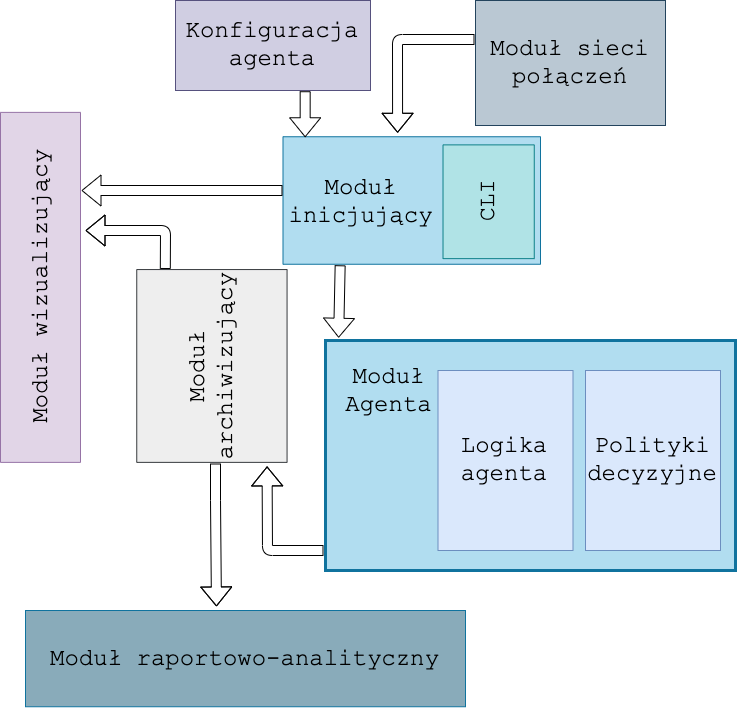
\includegraphics[width=\textwidth, height=0.7\textheight]{./system-arch.png}
	\caption{Architektura systemu z zaznaczanonymi modułami składowymi.}
	\label{arch1}
\end{figure}

\subsection{Moduł inicjujący}

Jest to moduł odpowiedzialny za inicjalizację wszystkich pozostałych składowych systemu oraz 
uruchomienie środowiska symulacji. Moduł ten:

\begin{itemize}

\item uruchamia moduł archiwizujący, w którym zapisywane są zdarzenia generowane przez agentów oraz stan systemu 
\item wczytuje z plików konfiguracyjnych strukturę połączeń między agentami oraz ich parametry wewnętrzne 
\item włącza interfejs graficzny   

\end{itemize}

\subsubsection{Wiersz poleceń}
\subsection{Moduł sieci połączeń}
\subsection{Moduł konfiguracyjny}
\subsection{Moduł Agenta}
\subsubsection{Logika agenta}
\subsubsection{Polityki decyzyjne}
\subsection{Moduł archiwizujący}
\subsection{Moduł wizualizujący}
\subsection{Moduł raportowo-analityczny}
\section{Symulacje \label{sec3}}
\subsection{Todo}
\subsection{Todo}
\subsection{Todo}
\subsection{Todo}
\subsection{Todo}
\end{document}
